\documentclass{beamer}
\usepackage{ulem}
\usepackage{tikz}
\usepackage{caption}
\usepackage{subcaption}
\usetikzlibrary{positioning}
\usetheme{Dresden}
\usecolortheme{wolverine}
\title{sMDT Chamber Production at the University of Michigan}
\author{Evan Carpenter}
\date{February 7th, 2023}

\definecolor{googlegreen}{rgb}{0.7137,0.8431,0.6588}
\definecolor{googleblue}{rgb}{0.4275,0.6196,0.9216}
\definecolor{googleyellow}{rgb}{1,1,0}
\definecolor{googlered}{rgb}{0.8784,0.4,0.4}
\setbeamertemplate{navigation symbols}{}
\addtobeamertemplate{navigation symbols}{}{%
    \usebeamerfont{footline}%
    \usebeamercolor[fg]{footline}%
    \hspace{1em}%
    \insertframenumber/\inserttotalframenumber
}

\def\ph{\textcolor{red}{PLACEHOLDER}}


\titlegraphic{
	\begin{tikzpicture}[remember picture, overlay]
		\node[xshift=-0.4\pdfpagewidth, yshift=0.05\pdfpageheight]{
\includegraphics[width=0.17\linewidth]{atlas.png}};
		\node [xshift=0.35\pdfpagewidth, yshift=0.031\pdfpageheight]{
\includegraphics[width=0.2\linewidth]{UM.png}};
	\end{tikzpicture}
}

\newcommand{\backupbegin}{
   \newcounter{finalframe}
   \setcounter{finalframe}{\value{framenumber}}
}
\newcommand{\backupend}{
   \setcounter{framenumber}{\value{finalframe}}
}

\begin{document}
\begin{frame}
	\titlepage
\end{frame}
\begin{frame}
	\tableofcontents
\end{frame}
\section*{Background and Overview}
	\begin{frame}
		word
	\end{frame}

	\begin{frame}{Chamber and Tube Construction}
		\begin{itemize}
			\item Goal is to produce 50 chambers total \textcolor{red}{(plus two extra?)}
			\item Last Muon week talk covered chambers 0-30
			\item Since then, chambers up to 35 have been fully made.
			\item Began construction of additional sMDTs in November to supplement chamber production.
			\item 2 papers published on methods. 
		\end{itemize}
	\end{frame}
	\section{UM Tube Production}
	\subsection{Construction Process}
		\begin{frame}{Overview}
			\begin{itemize}
				\item Started second wave of construction in November 2022 using station at UM.
				\item 4-5 full time workers would for construction and testing, 3 part time students for additional testing. 
				\item Goal of 1000 sMDTs constructed before 2023. Average 50 Tubes/Day. 
			\end{itemize}
		\end{frame}
		\begin{frame}{Construction and Testing}
			\begin{figure}
				\includegraphics[width=0.7\pdfpagewidth]{TubeProduction.png}
			\end{figure}
			\small Repurposing old station from last summer. 
			3-4 full time workers, 3 part time students. 
		\end{frame}
		\begin{frame}{Results}
			\begin{itemize}
				\item Completed after 32 working days in December 2022 with 1,352 tubes total. 
				\item Constructed sMDTs still undergoing QA/QC. 
				\item XX (check total number that need a good second tension as well) total failed. (Failure Rate of XX\%)
				\item 42 failed before full construction due to defects. 
			\end{itemize}
		\end{frame}
	\subsection{sMDT QA/QC Tests}
		\begin{frame}{QA Tests}
			\begin{figure}
				\begin{subfigure}[b]{0.25\pdfpagewidth}
					\includegraphics[width=0.25\pdfpagewidth]{LeakDetector.png}
					\caption{He Leak detector}
				\end{subfigure}
			\end{figure}
		\end{frame}
		\begin{frame}{Questions}
			\tableofcontents
		\end{frame}

\section{Chamber Production}
	\subsection{Construction Process}
		\begin{frame}

			\begin{description}
				\item [Week 1:] \colorbox{googlegreen}{Tube Gluing}
					\begin{itemize}\small
						\item Glue 2 layers per day (including gluing spacer frame/RASNIK layer)
					\end{itemize}
				\item [Week 2:] \colorbox{googlegreen}{AP Plate Mounting, Measurements.}
					\begin{itemize}\small
						\item Measure wire heights 
						\item Glue AP-plates, B-field sensors, CCC platforms.
						\item Measure platforms.
						\item Glue support bars.
					\end{itemize}
				\item [Week 3:] \colorbox{googleblue}{Gas Systems}
				\item [Week 4:] \colorbox{googleyellow}{Cosmic Ray Test}
			\end{description}
		\end{frame}
		\begin{frame}{\ph}
			\begin{figure}[t]
				\centering
				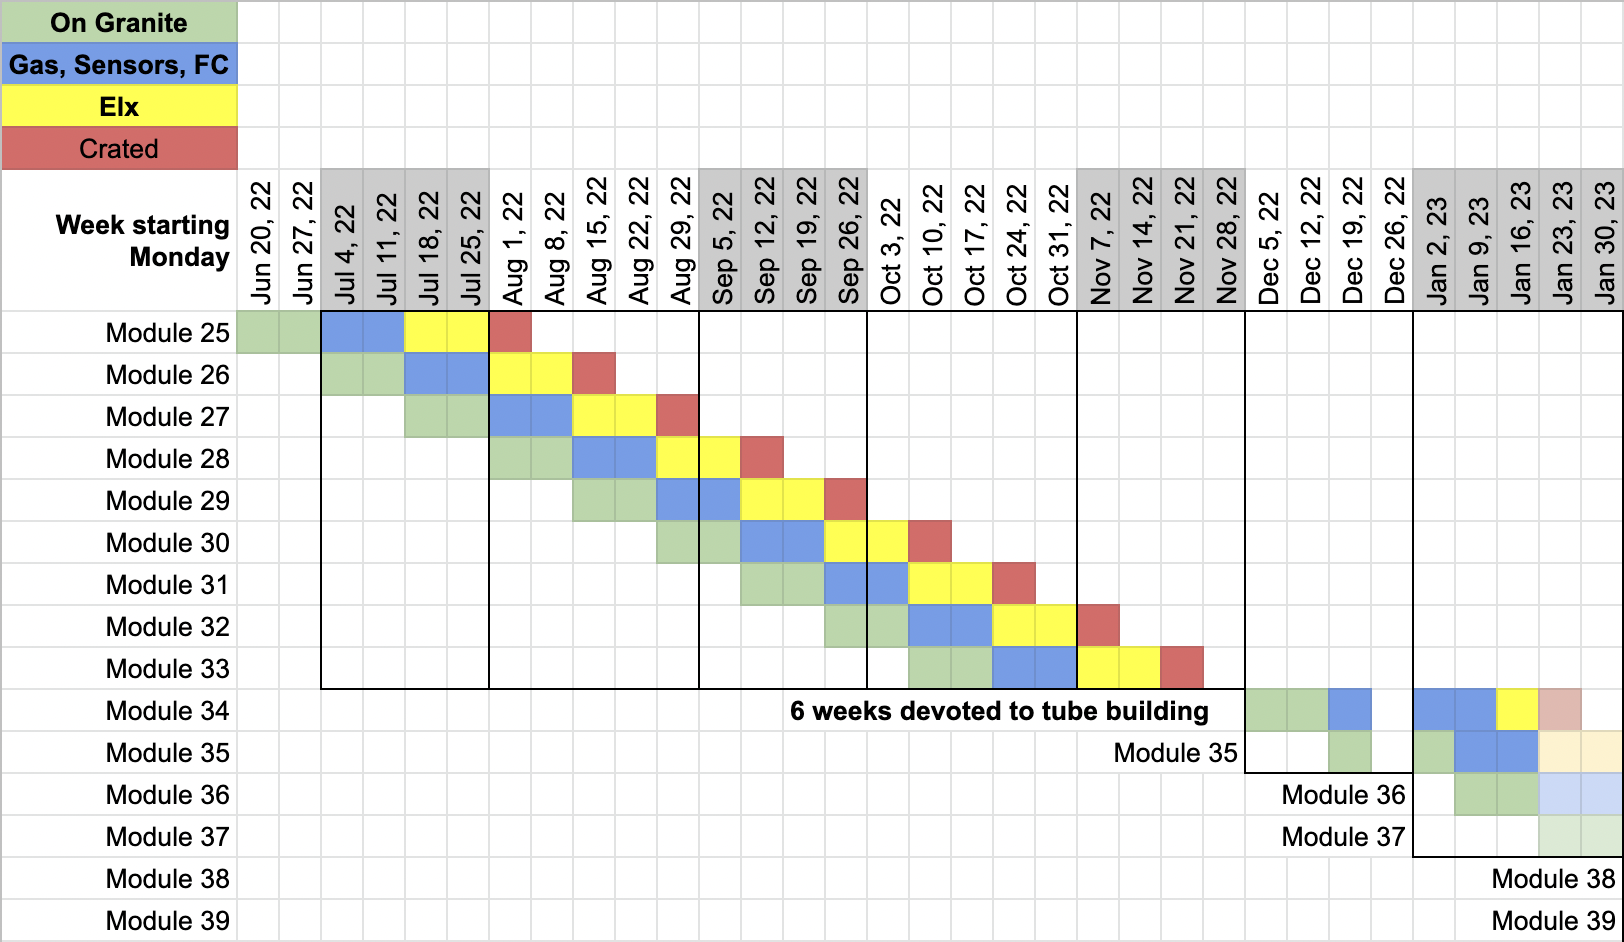
\includegraphics[width=0.8\pdfpagewidth]{Chamber Production.png}		
				\label{fig:ChamberProduction}		
			\end{figure}
		\end{frame}
	\subsection{Testing}

		\begin{frame}{Measurements \ph}
			\begin{itemize}
				\item Platform positioning / Endplug height positioning
				\item layer spacing layer pitch
				\item Leak Rate
				\item Effeciency
				\item Resolution
			\end{itemize}
		\end{frame}
		\begin{frame}{Wire Height \ph}
			\begin{figure}
				\centering
				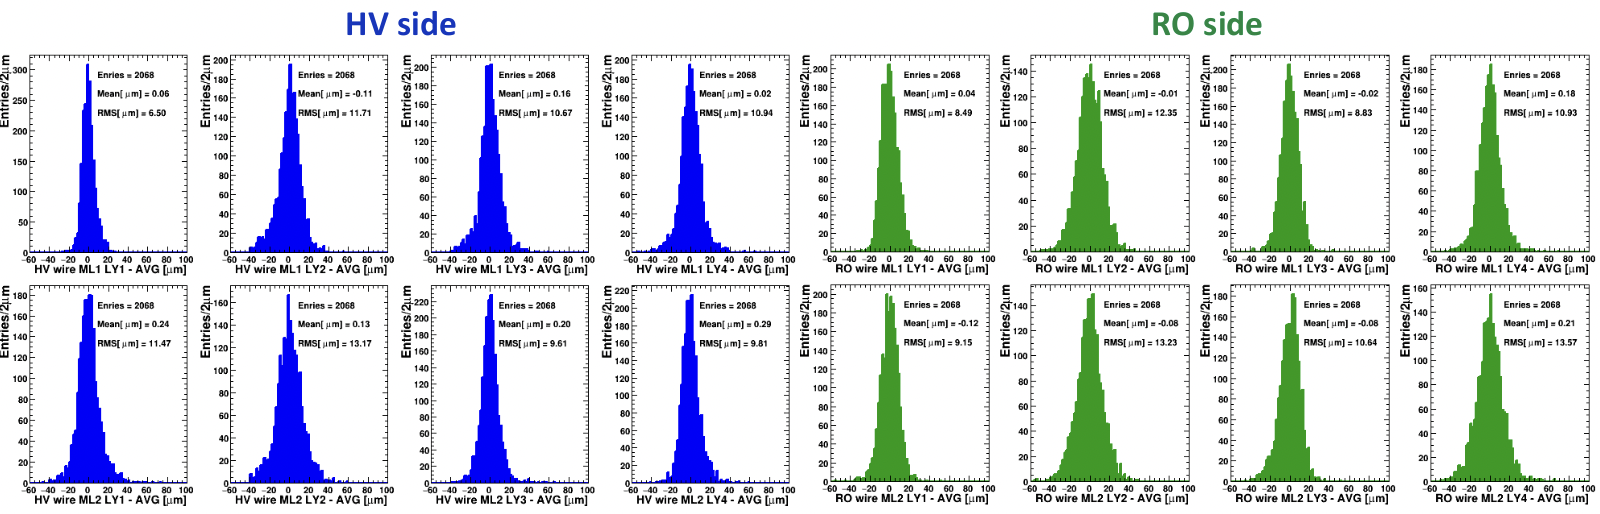
\includegraphics[width=0.8\pdfpagewidth]{WireHeightOffset.png}
			\end{figure}
		\end{frame}
		\begin{frame}{Inplane Alignment \ph}
			\begin{figure}[t]
				\centering	
				\begin{subfigure}[b]{0.4\pdfpagewidth}
					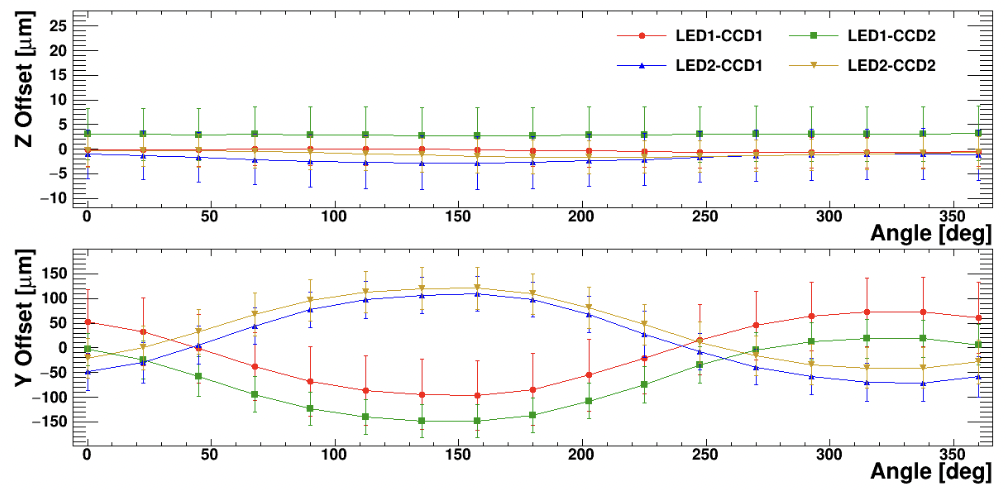
\includegraphics[width=0.4\pdfpagewidth]{RASNIKMeasurements.png}
					\caption{Deviation}
					\label{fig:InplaneAlignment}
				\end{subfigure}
			\end{figure}
		\end{frame}

		\begin{frame}{Leak Rate \ph}
			\begin{figure}
				\centering	
				\begin{subfigure}[c]{0.35\pdfpagewidth}
					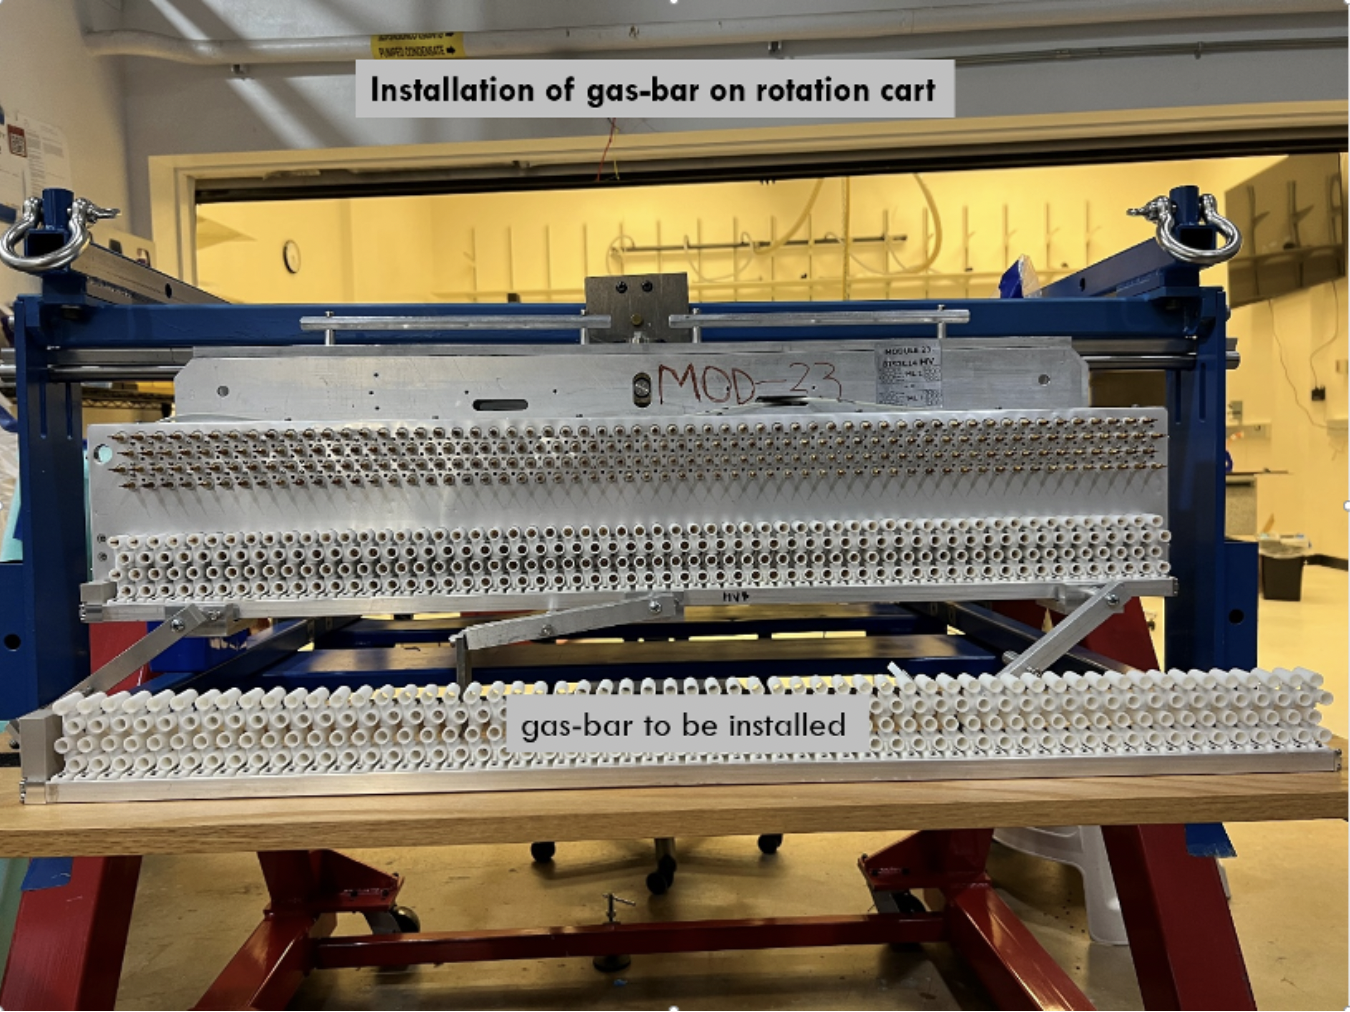
\includegraphics[width=0.35\pdfpagewidth]{GasBar.png}
					\caption{Chamber on rotation cart with gas bar to be installed}
				\end{subfigure}
				\hfill
				\begin{subfigure}[c]{0.4\pdfpagewidth}
					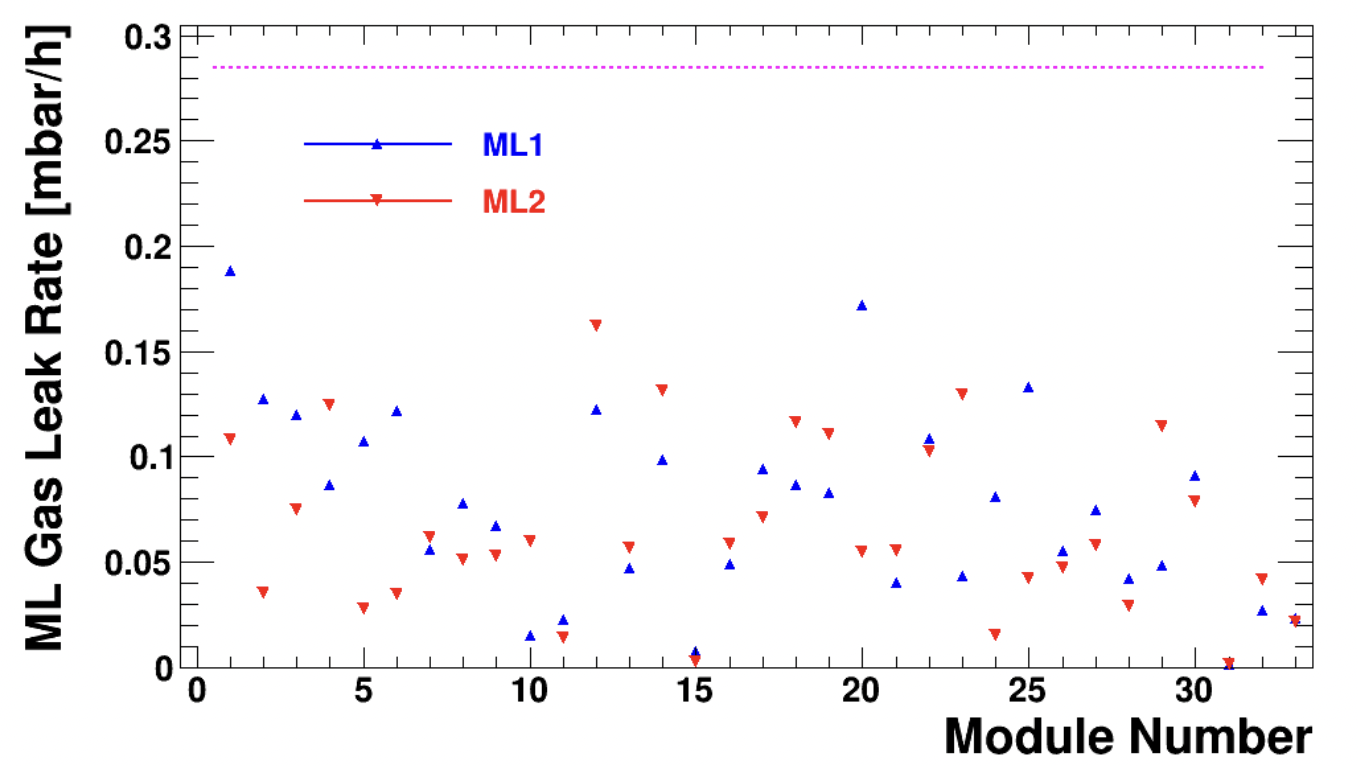
\includegraphics[width=0.4\pdfpagewidth]{ChamberLeakRate.png}
					\caption{Leak Rates of past 35 modules}
				\end{subfigure}
				\caption{hello}
			\end{figure}
		\end{frame}

		\begin{frame}{Efficiency \ph}
			\begin{figure}[t]
				\centering	
				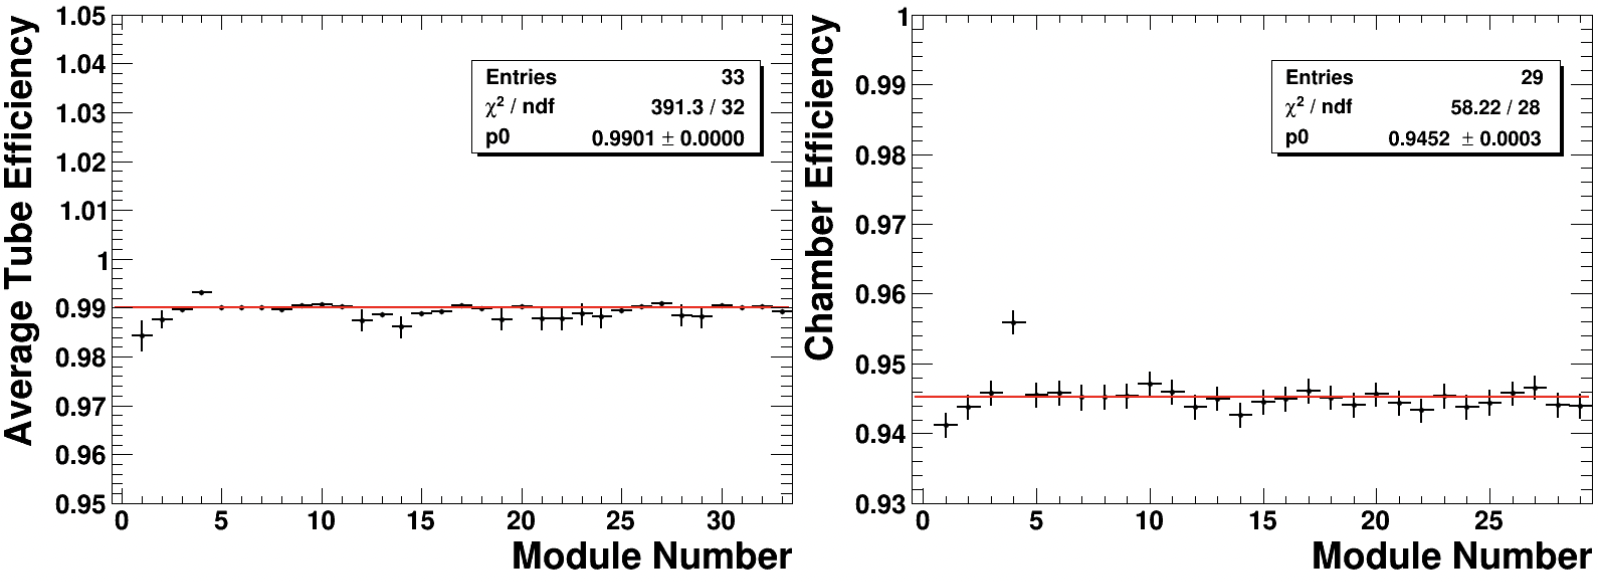
\includegraphics[width=0.8\pdfpagewidth]{ChamberEfficiency.png}
				\label{fig:ChamberEfficiency}
			\end{figure}
		\end{frame}
		
		\begin{frame}{Resolution \ph}
			\begin{figure}
				\centering	
				\begin{subfigure}[c]{0.4\pdfpagewidth}
					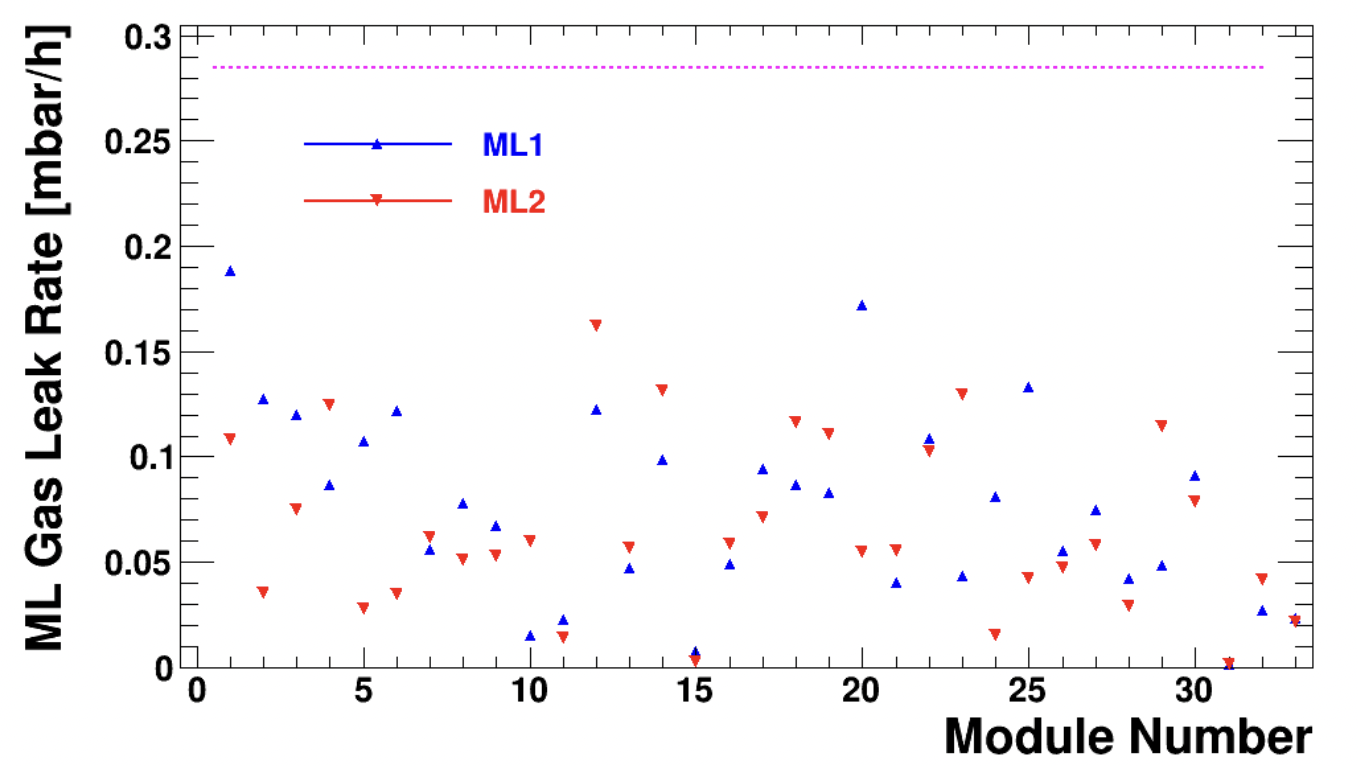
\includegraphics[width=0.3\pdfpagewidth]{ChamberLeakRate.png}
					\caption{INSERT PICTURE OF ELX}
				\end{subfigure}
				\hfill
				\begin{subfigure}[c]{0.4\pdfpagewidth}
					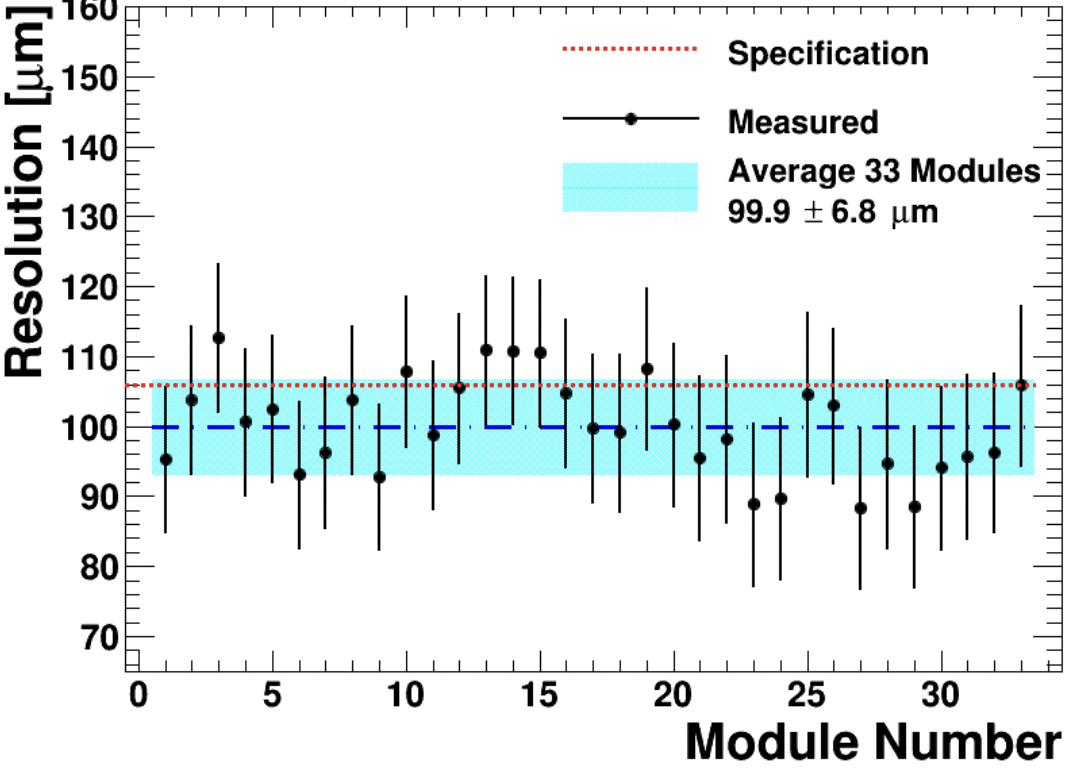
\includegraphics[width=0.4\pdfpagewidth]{ChamberResolution.png}
					\caption{Resolution}
					\label{fig:ChamberResolution}
				\end{subfigure}
			\end{figure}
			
		\end{frame}



	\subsection{Moving Forward}

		\begin{frame}{New Electronics}
		\end{frame}




\appendix
\backupbegin
\section{Extra}
	\begin{frame}
		\centering\Huge EXTRA SLIDES
	\end{frame}
	\begin{frame}{Leak Rate - Extra}
		\begin{figure}
			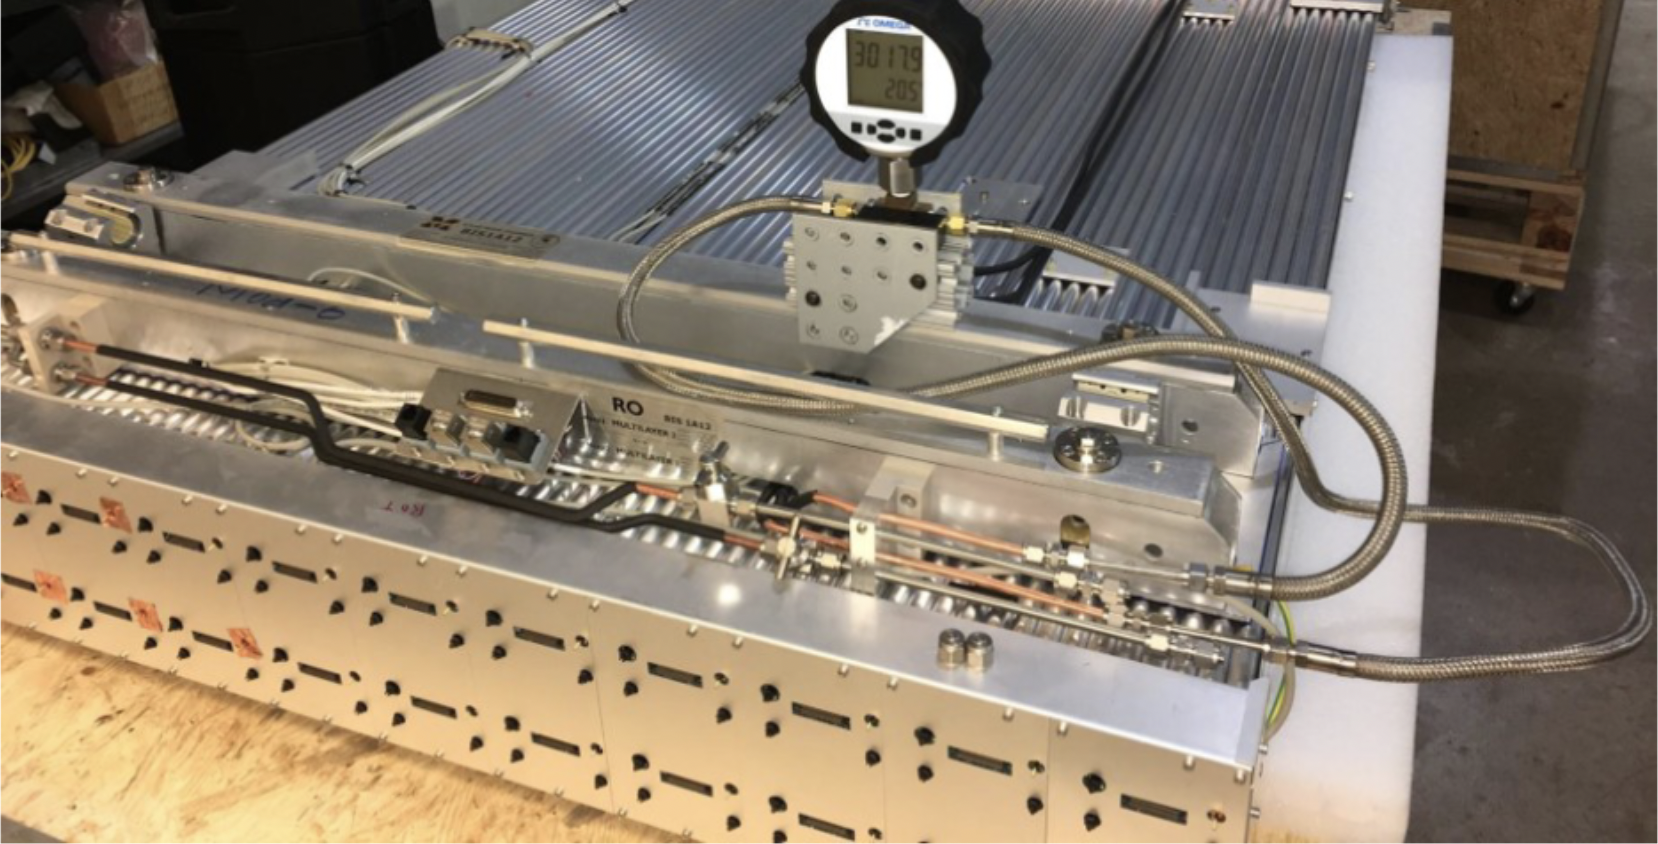
\includegraphics[width=0.5\pdfpagewidth]{PressureGauge.png}
		\end{figure}
		$$\Delta P_\text{corr}=P_f\frac{T_\text{ref}}{T_f}-P_i\frac{T_\text{ref}}{T_i}$$
	\end{frame}
	\begin{frame}{Detailed UM Failure Rate}
		\begin{itemize}
			\item 34 raw tubes failed due to dent or deformities that prevented construction. 
			\item 8 failed due to construction/mechanical errors that were seperate from normal testing.
		\end{itemize}
	\end{frame}
	\begin{frame}{DC Test - Extra}
		words
	\end{frame}
	\begin{frame}{Tension Test - Extra}
		Tension test is performed with LabVIEW.
	\end{frame}
\backupend
\end{document}